\section{Software Process Model}

SmartExam is a twelve-module platform with interdependent components, evolving design decisions, and iterative supervisor feedback. Waterfall does not work here. A model that locks requirements on day one and delivers working software on the last day would leave too many design assumptions untested for too long.

We chose Agile because it fits the nature of this project: complex enough to need structured sprints, but uncertain enough to benefit from continuous review and correction.

\subsection{Process Model Introduction}

Agile divides development into short, focused cycles called sprints. Each sprint produces working, demonstrable software. If a design decision turns out to be wrong — say, the invigilator dashboard is too cluttered — it is caught and fixed in the next sprint rather than discovered at the final demonstration.

This matters particularly for SmartExam. Role-based dashboards, HWID binding logic, and live telemetry streaming all interact. Getting the interaction right requires building early, testing with real users, and refining based on what breaks. Agile creates the structure to do this systematically. Figure~\ref{fig:agileworkflowdetailed} shows the sprint cycle, feedback loops, and supervisor review milestones.

\begin{figure}[H]
\centering
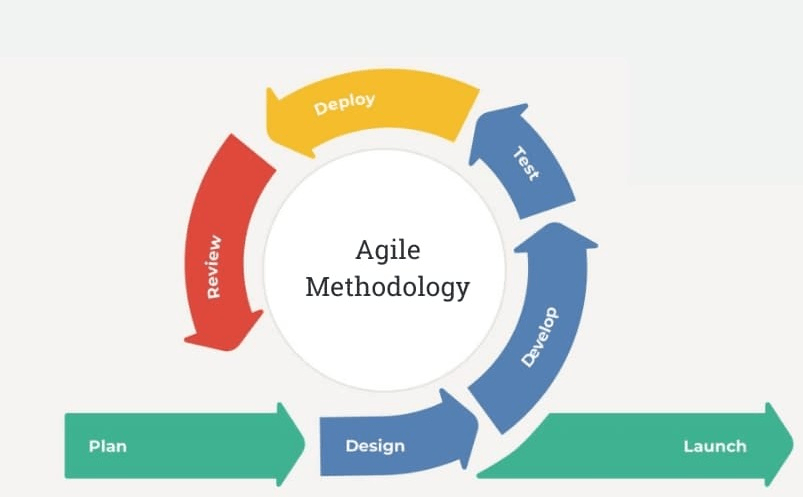
\includegraphics[width=0.97\linewidth]{Figures/agile_workflow_detailed.png}
\caption{Detailed Agile Workflow with Sprint Feedback and Review Loops}
\label{fig:agileworkflowdetailed}
\end{figure}

\subsection{Justification of Proposing the Process Model}

The twelve modules of SmartExam do not all have equal certainty at the start. Authentication and role management are well-understood. Face recognition integration, live WebSocket telemetry synchronisation, and AI theory grading carry more design risk. A sequential model forces the team to specify these uncertain components fully before writing a line of code. That is unrealistic.

Agile splits the risk. High-certainty modules ship first. Uncertain modules get prototyped early and refined across multiple sprints before integration. Supervisor feedback from prototype reviews shapes later sprints without destabilising earlier work. This approach also matches the FYP timeline. Academic review happens at mid-semester and end-of-semester milestones — exactly the rhythm Agile sprint reviews follow.

\subsection{Steps of Process Model}

Eight sprints cover the full project, each running for four weeks. The twelve modules are distributed so that every sprint delivers a meaningful, reviewable increment.

\textbf{Sprint 1 (Weeks 1--4):} Requirement Analysis and System Planning. Activities include stakeholder interviews, use-case mapping, product backlog creation, initial architecture design, and scope approval from the supervisor.

\textbf{Sprint 2 (Weeks 5--8):} Core Access Control and Authentication. Delivers Module 1 (Authentication and Device Binding) and Module 7 (User and Role Management). The team builds JWT login endpoints, HWID extraction via WMI API calls, user registration screens, and role-based dashboard routing.

\textbf{Sprint 3 (Weeks 9--12):} Exam Configuration and Administration. Delivers Module 8 (Exam Creation and Configuration) and Module 9 (Eligibility and Access Control). The team builds exam templates, application blocklists, test-case definitions, and seat assignment logic.

\textbf{Sprint 4 (Weeks 13--16):} Student Desktop Client Environment. Delivers Module 2 (Pre-Exam Verification), Module 3 (Exam Dashboard), and Module 4 (Secure Exam Environment). The WPF client launches in fullscreen, disabling Alt+Tab and Task Manager. Hardware readiness checks run before the session begins.

\textbf{Sprint 5 (Weeks 17--20):} Live Telemetry and Proctoring. Delivers Module 5 (Live Monitoring Client Service) and Module 10 (Live Proctoring Dashboard). Background services log focus switches and process lists every few seconds. A SignalR WebSocket connection streams this data to the React-based teacher dashboard.

\textbf{Sprint 6 (Weeks 21--24):} Submission and AI Evaluation. Delivers Module 6 (Submission and Backup) and Module 11 (AI-Assisted Evaluation). The team implements auto-save with local encrypted backups, isolated code compilation against test cases, and AI semantic scoring for theory answers. A class-wide plagiarism comparison matrix is generated at submission close.

\textbf{Sprint 7 (Weeks 25--28):} Reporting, Analytics, and Auditing. Delivers Module 12 (Logs, Analytics and Audit Trail). The team builds immutable audit log tables, system performance dashboards, and QuestPDF-based downloadable exam reports.

\textbf{Sprint 8 (Weeks 29--32):} Integration, Testing, and Final Refinement. No new modules. This sprint merges all twelve modules into one stable prototype, runs end-to-end tests, fixes integration bugs, and prepares the final academic submission and demonstration.
